% KI-Übersetzung in modernes Deutsch nach der zugrunde gelegten LaTeX-Transkription der Druckseiten 202--211 einschließlich der unnummerierten Seite [205].
\begingroup
\clearpage
\noindent202\hfill\textsc{Bemerkungen.}\hfill\mbox{}\par\medskip
\begingroup\footnotesize
\[
\begin{array}{r@{\qquad}l}
2)&\displaystyle \tfrac1{12}\frac{(1-ee\sin\varphi^2)^3}{a^4(1-ee)^3}
\{1-3ee+(ee+15e^4)\sin\varphi^2-14e^4\sin\varphi^4\}=\beta,
\end{array}
\]
so ist nach Art.~[7], S.~154:
\[
\log n=\alpha yy-\beta y^4+\cdots.
\]
Es sei $x$ nach Süden positiv, so dass
\[
\begin{array}{r@{\qquad}l}
3)&\displaystyle\frac{\partial\alpha}{\partial x}
=\frac{\partial\alpha}{\partial\varphi}.\frac{\mathrm d\varphi}{\mathrm dx}
=+\frac{ee\sin2\varphi(1-ee\sin\varphi^2)^{\frac52}}{a^3(1-ee)^2}=\gamma
\end{array}
\]
wird. Für einen Punkt $x+x'$, $y+y'$ ist mithin:
\[
\begin{aligned}
\log n&=(\alpha+\gamma x'+\cdots)(yy+2yy'+y'y')-(\beta+\cdots)(y^4+4y^3y'+\cdots)+\cdots\\
&=\alpha yy-\beta y^4+\cdots+(\gamma yy-\cdots)x'+(2\alpha y-4\beta y^3+\cdots)y'\cdots.
\end{aligned}
\]
Also ist nach [16], S.~165, mit der angegebenen Vernachlässigung:
\[
A=\gamma yy,\qquad B=2\alpha y-4\beta y^3.
\]
Folglich wird für den Punkt, dessen Koordinaten
\[
\begin{gathered}
x_1+\tfrac13(x_2-x_1)=\xi\\
y_1+\tfrac13(y_2-y_1)=\eta
\end{gathered}
\]
sind:
\[
A_{\frac13}=\gamma\eta\eta,\qquad B_{\frac13}=2\alpha\eta-4\beta\eta^3,
\]
wobei jetzt $\alpha$, $\beta$, $\gamma$ zur Abszisse $\xi$ gehören.

Damit ergibt sich aber für $\psi$:
\[
\psi=(\alpha\eta-2\beta\eta^3)(x_2-x_1)-\tfrac12\gamma\eta\eta(y_2-y_1)
\]
oder
\[
\begin{array}{r@{\qquad}l}
4)&-\psi=-\alpha\eta(x_2-x_1)+2\beta\eta^3(x_2-x_1)+\tfrac12\gamma\eta\eta(y_2-y_1).
\end{array}
\]
$\alpha$, $2\beta$, $\tfrac12\gamma$ sind dieselben Größen wie $\alpha$, $\beta$, $\gamma$ auf S.~159.
\begin{center}\rule{4cm}{.4pt}\end{center}
\bigskip
Anstelle der Formeln für die \textsc{Mercator}-Projektion bei der Übertragung der Kugelfläche in der Ebene, Art.~[29], S.~185, kann man sich auch der Formeln des Art.~[13] bedienen, wenn man in ihnen $\delta=0$ setzt. Gehört zu dem Punkt $x'$, $y'$ in der Ebene der Punkt $\Omega$, $\lambda$ auf der Kugel, so ist der Gleichung
\[
x'+iy'=\mathrm g(\mathrm F(\Omega)+i\lambda),\qquad
\mathrm F(\Omega)=\int\frac{\mathrm d\Omega}{\cos\Omega}
=\log\operatorname{hyp}\operatorname{tang}(45^\circ+\tfrac12\Omega),
\]
entsprechend, wenn jetzt $x'$ nach Norden positiv genommen wird, und wenn unter $\omega$ der Meridianbogen vom Äquator bis zur Breite $\Omega$ verstanden wird $\left(\omega=10000000.\frac{\Omega^\circ}{90^\circ}\right)$:
\[
\begin{aligned}
x'&=\omega+\frac r4\sin2\Omega.\lambda\lambda+\frac r{48}\sin2\Omega(6\cos\Omega^2-1)\lambda^4\cdots\\
y'&=r\cos\Omega.\lambda+\frac r6\cos\Omega\cos2\Omega.\lambda^3
+\frac r{120}\cos\Omega(1-20\cos\Omega^2+24\cos\Omega^4)\lambda^5\cdots;
\end{aligned}
\]
\[
r=\frac{20000000}{\pi}.
\]
\par\endgroup
\clearpage
\noindent\mbox{}\hfill\textsc{Konforme Abbildung des Sphäroids in der Ebene.}\hfill203\par\medskip
\begingroup\footnotesize
Für
\[
\begin{array}{rcl@{\qquad}rcl}
\Omega&=&53^\circ13'3''{,}6353&\lambda&=&1^\circ48'24''{,}7109=6504''{,}7109\\
2\Omega&=&106\quad26\quad7{,}2706&&&
\end{array}
\]
ist
\begin{center}
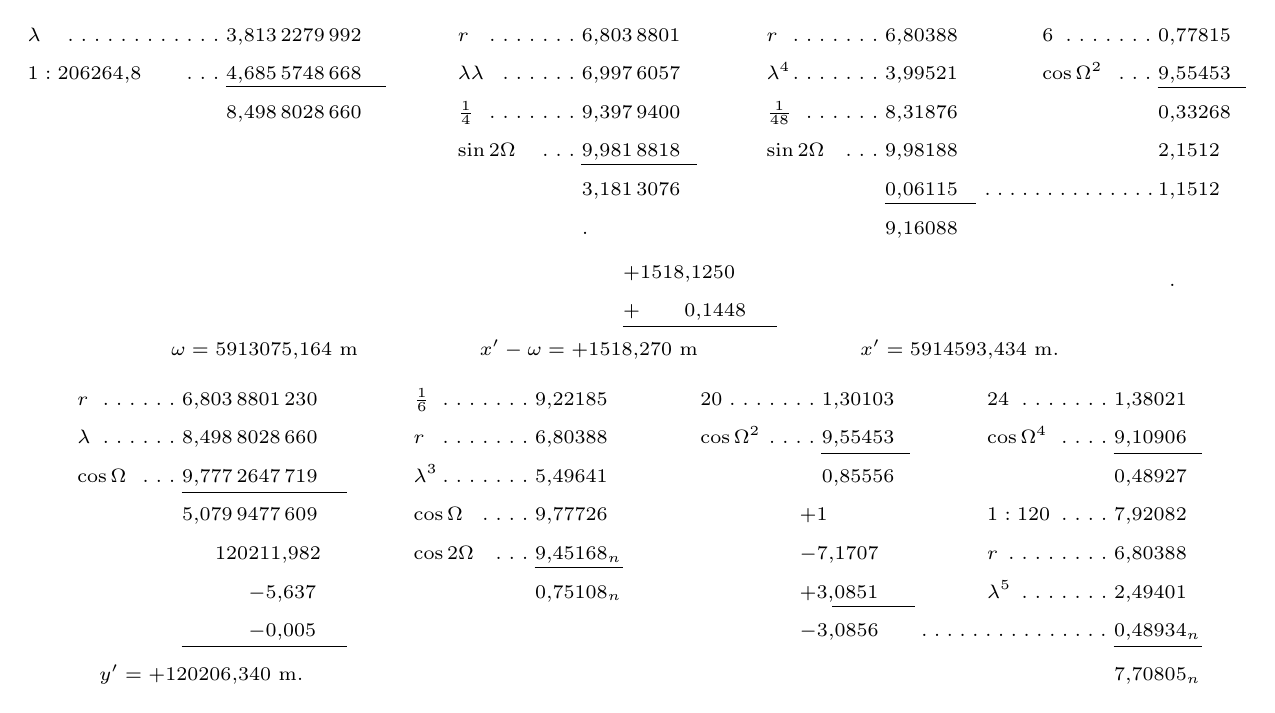
\begin{tikzpicture}[x=.007cm,y=-.007cm,every node/.style={anchor=base west,inner sep=0pt,font=\fontsize{7.5}{9}\selectfont},line width=.3pt]
\node at (0,0) {$\lambda$};
\node at (72,0) {$.$};
\node at (96,0) {$.$};
\node at (120,0) {$.$};
\node at (144,0) {$.$};
\node at (168,0) {$.$};
\node at (192,0) {$.$};
\node at (216,0) {$.$};
\node at (240,0) {$.$};
\node at (264,0) {$.$};
\node at (288,0) {$.$};
\node at (312,0) {$.$};
\node at (336,0) {$.$};
\node at (360,0) {$3{,}813\,2279\,992$};
\node at (0,70) {$1:206264{,}8$};
\node at (288,70) {$.$};
\node at (312,70) {$.$};
\node at (336,70) {$.$};
\node at (360,70) {$4{,}685\,5748\,668$};
\draw (360,82)--(650,82);
\node at (360,140) {$8{,}498\,8028\,660$};
\node at (780,0) {$r$};
\node at (837,0) {$.$};
\node at (861,0) {$.$};
\node at (885,0) {$.$};
\node at (909,0) {$.$};
\node at (933,0) {$.$};
\node at (957,0) {$.$};
\node at (981,0) {$.$};
\node at (1005,0) {$6{,}803\,8801$};
\node at (780,70) {$\lambda\lambda$};
\node at (861,70) {$.$};
\node at (885,70) {$.$};
\node at (909,70) {$.$};
\node at (933,70) {$.$};
\node at (957,70) {$.$};
\node at (981,70) {$.$};
\node at (1005,70) {$6{,}997\,6057$};
\node at (780,140) {$\frac14$};
\node at (837,140) {$.$};
\node at (861,140) {$.$};
\node at (885,140) {$.$};
\node at (909,140) {$.$};
\node at (933,140) {$.$};
\node at (957,140) {$.$};
\node at (981,140) {$.$};
\node at (1005,140) {$9{,}397\,9400$};
\node at (780,210) {$\sin2\Omega$};
\node at (933,210) {$.$};
\node at (957,210) {$.$};
\node at (981,210) {$.$};
\node at (1005,210) {$9{,}981\,8818$};
\draw (1005,224)--(1215,224);
\node at (1005,280) {$3{,}181\,3076$};
\node at (1340,0) {$r$};
\node at (1387,0) {$.$};
\node at (1411,0) {$.$};
\node at (1435,0) {$.$};
\node at (1459,0) {$.$};
\node at (1483,0) {$.$};
\node at (1507,0) {$.$};
\node at (1531,0) {$.$};
\node at (1555,0) {$6{,}80388$};
\node at (1340,70) {$\lambda^4$};
\node at (1387,70) {$.$};
\node at (1411,70) {$.$};
\node at (1435,70) {$.$};
\node at (1459,70) {$.$};
\node at (1483,70) {$.$};
\node at (1507,70) {$.$};
\node at (1531,70) {$.$};
\node at (1555,70) {$3{,}99521$};
\node at (1340,140) {$\frac1{48}$};
\node at (1411,140) {$.$};
\node at (1435,140) {$.$};
\node at (1459,140) {$.$};
\node at (1483,140) {$.$};
\node at (1507,140) {$.$};
\node at (1531,140) {$.$};
\node at (1555,140) {$8{,}31876$};
\node at (1340,210) {$\sin2\Omega$};
\node at (1483,210) {$.$};
\node at (1507,210) {$.$};
\node at (1531,210) {$.$};
\node at (1555,210) {$9{,}98188$};
\node at (1555,280) {$0{,}06115$};
\draw (1555,295)--(1720,295);
\node at (1555,350) {$9{,}16088$};
\node at (1840,0) {$6$};
\node at (1882,0) {$.$};
\node at (1906,0) {$.$};
\node at (1930,0) {$.$};
\node at (1954,0) {$.$};
\node at (1978,0) {$.$};
\node at (2002,0) {$.$};
\node at (2026,0) {$.$};
\node at (2050,0) {$0{,}77815$};
\node at (1840,70) {$\cos\Omega^2$};
\node at (1978,70) {$.$};
\node at (2002,70) {$.$};
\node at (2026,70) {$.$};
\node at (2050,70) {$9{,}55453$};
\draw (2050,84)--(2210,84);
\node at (2050,140) {$0{,}33268$};
\node at (2050,210) {$2{,}1512$};
\node at (2050,280) {$1{,}1512$};
\node at (1735.00,280) {$.$};
\node at (1757.69,280) {$.$};
\node at (1780.38,280) {$.$};
\node at (1803.08,280) {$.$};
\node at (1825.77,280) {$.$};
\node at (1848.46,280) {$.$};
\node at (1871.15,280) {$.$};
\node at (1893.85,280) {$.$};
\node at (1916.54,280) {$.$};
\node at (1939.23,280) {$.$};
\node at (1961.92,280) {$.$};
\node at (1984.62,280) {$.$};
\node at (2007.31,280) {$.$};
\node at (2030.00,280) {$.$};
\node at (1005,350) {$.$};
\node at (2070,445) {$.$};
\node at (1080,430) {$+1518{,}1250$};
\node at (1080,500) {$+\phantom{1518}0{,}1448$};
\draw (1080,518)--(1360,518);
\node at (260,570) {$\omega=5913075{,}164\ \mathrm m$};
\node at (820,570) {$x'-\omega=+1518{,}270\ \mathrm m$};
\node at (1510,570) {$x'=5914593{,}434\ \mathrm m.$};

\node at (90,660) {$r$};
\node at (136,660) {$.$};
\node at (160,660) {$.$};
\node at (184,660) {$.$};
\node at (208,660) {$.$};
\node at (232,660) {$.$};
\node at (256,660) {$.$};
\node at (280,660) {$6{,}803\,8801\,230$};
\node at (90,730) {$\lambda$};
\node at (136,730) {$.$};
\node at (160,730) {$.$};
\node at (184,730) {$.$};
\node at (208,730) {$.$};
\node at (232,730) {$.$};
\node at (256,730) {$.$};
\node at (280,730) {$8{,}498\,8028\,660$};
\node at (90,800) {$\cos\Omega$};
\node at (208,800) {$.$};
\node at (232,800) {$.$};
\node at (256,800) {$.$};
\node at (280,800) {$9{,}777\,2647\,719$};
\draw (280,818)--(580,818);
\node at (280,870) {$5{,}079\,9477\,609$};
\node at (340,940) {$120211{,}982$};
\node at (400,1010) {$-5{,}637$};
\node at (400,1080) {$-0{,}005$};
\draw (280,1098)--(580,1098);
\node at (130,1160) {$y'=+120206{,}340\ \mathrm m.$};
\node at (700,660) {$\frac16$};
\node at (752,660) {$.$};
\node at (776,660) {$.$};
\node at (800,660) {$.$};
\node at (824,660) {$.$};
\node at (848,660) {$.$};
\node at (872,660) {$.$};
\node at (896,660) {$.$};
\node at (920,660) {$9{,}22185$};
\node at (700,730) {$r$};
\node at (752,730) {$.$};
\node at (776,730) {$.$};
\node at (800,730) {$.$};
\node at (824,730) {$.$};
\node at (848,730) {$.$};
\node at (872,730) {$.$};
\node at (896,730) {$.$};
\node at (920,730) {$6{,}80388$};
\node at (700,800) {$\lambda^3$};
\node at (752,800) {$.$};
\node at (776,800) {$.$};
\node at (800,800) {$.$};
\node at (824,800) {$.$};
\node at (848,800) {$.$};
\node at (872,800) {$.$};
\node at (896,800) {$.$};
\node at (920,800) {$5{,}49641$};
\node at (700,870) {$\cos\Omega$};
\node at (824,870) {$.$};
\node at (848,870) {$.$};
\node at (872,870) {$.$};
\node at (896,870) {$.$};
\node at (920,870) {$9{,}77726$};
\node at (700,940) {$\cos2\Omega$};
\node at (848,940) {$.$};
\node at (872,940) {$.$};
\node at (896,940) {$.$};
\node at (920,940) {$9{,}45168_n$};
\draw (920,955)--(1080,955);
\node at (920,1010) {$0{,}75108_n$};
\node at (1220,660) {$20$};
\node at (1272,660) {$.$};
\node at (1296,660) {$.$};
\node at (1320,660) {$.$};
\node at (1344,660) {$.$};
\node at (1368,660) {$.$};
\node at (1392,660) {$.$};
\node at (1416,660) {$.$};
\node at (1440,660) {$1{,}30103$};
\node at (1220,730) {$\cos\Omega^2$};
\node at (1344,730) {$.$};
\node at (1368,730) {$.$};
\node at (1392,730) {$.$};
\node at (1416,730) {$.$};
\node at (1440,730) {$9{,}55453$};
\draw (1440,748)--(1600,748);
\node at (1440,800) {$0{,}85556$};
\node at (1400,870) {$+1$};
\node at (1400,940) {$-7{,}1707$};
\node at (1400,1010) {$+3{,}0851$};
\draw (1460,1025)--(1610,1025);
\node at (1400,1080) {$-3{,}0856$};
\node at (1740,660) {$24$};
\node at (1802,660) {$.$};
\node at (1826,660) {$.$};
\node at (1850,660) {$.$};
\node at (1874,660) {$.$};
\node at (1898,660) {$.$};
\node at (1922,660) {$.$};
\node at (1946,660) {$.$};
\node at (1970,660) {$1{,}38021$};
\node at (1740,730) {$\cos\Omega^4$};
\node at (1874,730) {$.$};
\node at (1898,730) {$.$};
\node at (1922,730) {$.$};
\node at (1946,730) {$.$};
\node at (1970,730) {$9{,}10906$};
\draw (1970,748)--(2130,748);
\node at (1970,800) {$0{,}48927$};
\node at (1740,870) {$1:120$};
\node at (1874,870) {$.$};
\node at (1898,870) {$.$};
\node at (1922,870) {$.$};
\node at (1946,870) {$.$};
\node at (1970,870) {$7{,}92082$};
\node at (1740,940) {$r$};
\node at (1778,940) {$.$};
\node at (1802,940) {$.$};
\node at (1826,940) {$.$};
\node at (1850,940) {$.$};
\node at (1874,940) {$.$};
\node at (1898,940) {$.$};
\node at (1922,940) {$.$};
\node at (1946,940) {$.$};
\node at (1970,940) {$6{,}80388$};
\node at (1740,1010) {$\lambda^5$};
\node at (1802,1010) {$.$};
\node at (1826,1010) {$.$};
\node at (1850,1010) {$.$};
\node at (1874,1010) {$.$};
\node at (1898,1010) {$.$};
\node at (1922,1010) {$.$};
\node at (1946,1010) {$.$};
\node at (1970,1010) {$2{,}49401$};
\node at (1970,1080) {$0{,}48934_n$};
\draw (1970,1098)--(2130,1098);
\node at (1970,1160) {$7{,}70805_n$};
\node at (1620.00,1080) {$.$};
\node at (1643.21,1080) {$.$};
\node at (1666.43,1080) {$.$};
\node at (1689.64,1080) {$.$};
\node at (1712.86,1080) {$.$};
\node at (1736.07,1080) {$.$};
\node at (1759.29,1080) {$.$};
\node at (1782.50,1080) {$.$};
\node at (1805.71,1080) {$.$};
\node at (1828.93,1080) {$.$};
\node at (1852.14,1080) {$.$};
\node at (1875.36,1080) {$.$};
\node at (1898.57,1080) {$.$};
\node at (1921.79,1080) {$.$};
\node at (1945.00,1080) {$.$};
\end{tikzpicture}
\end{center}
\begin{center}\rule{4cm}{.4pt}\end{center}
Zu Art.~[30] sei bemerkt: Die \textsc{Gauss}sche Logarithmentafel (v.~\textsc{Zachs} Monatliche Correspondenz. XXVI.~Band. Gotha 1812, S.~498---528) gibt
\[
\mathrm A=\log n,\qquad\mathrm B=\log\left(1+\frac1n\right),\qquad
\mathrm C=\log(1+n),
\]
wo $n$ eine positive Zahl bedeutet. $\mathrm A+\mathrm B=\mathrm C$.

Setzt man $\mathrm C=2\log\sec\psi=\frac{k\pi y}{10^7}$, so wird $\mathrm A=2\log\operatorname{tang}\psi$, $\mathrm B=-2\log\sin\psi$. Setzt man $\mathrm B=2\log\sec\psi=\frac{k\pi y}{10^7}$, so wird $\mathrm A=-2\log\operatorname{tang}\psi$, $\mathrm C=-2\log\sin\psi$. Damit findet man die angegebenen Werte für $\log\frac{\sin iy}{i}=\log\frac{\sin\psi^2}{2\cos\psi}$.
\begin{center}\rule{4cm}{.4pt}\end{center}
\bigskip
Die beiden Formeln unter [32] erhält man wie folgt.

Setzt man $\Phi=90^\circ-p$, so ist nach 2) und 3), S.~199, wenn der Anfangspunkt der Koordinaten einem bestimmten Punkt des Hauptmeridians entspricht:
\[
\begin{array}{r@{\qquad}l}
1)&\displaystyle\mathrm f(\xi)=\log\operatorname{hyp}
\left(\operatorname{cotang}\frac p2.\left(\frac{1-e\cos p}{1+e\cos p}\right)^{\frac12e}\right)-K,
\end{array}
\]
\par\endgroup
\vfill\noindent\hfill26\textsuperscript{$\ast$}\hspace*{2cm}
\clearpage
\noindent204\hfill\textsc{Bemerkungen. Konforme Abbildung des Sphäroids in der Ebene.}\par\medskip
\begingroup\footnotesize
wo $K$ der Wert des Logarithmus für den Anfangspunkt ist, sodass
\[
\mathrm f(\xi)+i\lambda=\log\operatorname{hyp}\left\{\operatorname{cotang}\frac p2.\left(\frac{1-e\cos p}{1+e\cos p}\right)^{\frac12e}.(\cos\lambda+i\sin\lambda)\right\}-K.
\]
Dabei ist $\xi$ auch die Länge des Meridianbogens vom Anfangspunkt bis zur Breite $90^\circ-p$, der ebenso wie die Abszissen nach Süden positiv gezählt werden soll. Mithin ist
\[
\begin{array}{r@{\qquad}l}
2)&\displaystyle\xi=\int\frac{a(1-ee)\,\mathrm dp}{\sqrt{(1-ee\cos p^2)^3}}.
\end{array}
\]
Setzt man nun
\[
\begin{array}{r@{\quad}l}
3)&\displaystyle\operatorname{cotang}\frac P2.\left(\frac{1-e\cos P}{1+e\cos P}\right)^{\frac12e}
=\operatorname{cotang}\frac p2.\left(\frac{1-e\cos p}{1+e\cos p}\right)^{\frac12e}.(\cos\lambda+i\sin\lambda),
\end{array}
\]
wobei für $\lambda=0$: $P=p$, sowie $y=0$ und $x=\xi$ ist, so wird wegen $\mathrm f(\xi)+i\lambda=\mathrm f(x+iy)$:
\[
\begin{array}{r@{\qquad}l}
4)&\displaystyle\mathrm f(x+iy)=\log\operatorname{hyp}\left(\operatorname{cotang}\frac P2.\left(\frac{1-e\cos P}{1+e\cos P}\right)^{\frac12e}\right)-K;
\end{array}
\]
folglich muss der Gleichung 2) entsprechend:
\[
\begin{array}{r@{\qquad}l}
5)&\displaystyle x+iy=\int\frac{a(1-ee)\,\mathrm dP}{\sqrt{(1-ee\cos P)^3}}
\end{array}
\]
sein.
\begin{center}\rule{4cm}{.4pt}\end{center}
\bigskip
Die Entwicklungen zu den Artikeln [1]--[15], [21] und [22] sind wahrscheinlich in der Zeit zwischen 1816 und 1820 entstanden, während die übrigen Artikel aus den Jahren 1825--1827 zu stammen scheinen.
\begin{flushright}\textsc{Krüger.}\end{flushright}
\begin{center}\rule{7cm}{.5pt}\end{center}
\par\endgroup
\clearpage
% The source opening leaf [205] has no printed folio or running header.
\vspace*{1.3cm}
\begin{center}
{\Large\bfseries BRIEFWECHSEL.}\par
\vspace{1.7cm}
{\large\bfseries [Über die Formeln für die hannoversche Landesvermessung.]}\par
\bigskip
\textsc{Gauss} an \textsc{Schumacher}.\quad Göttingen, 18.~April 1830.
\end{center}
\medskip
.\ .\ .\ .\ .\ .\ Es scheint mir bei Ihren Messungen, insofern Sie sich auf eine der beiden in meinem früheren Brief erörterten Methoden beschränken wollen, am angemessensten, wenn Sie Ihre Resultate für die Lage der einzelnen Punkte in Koordinatenform berechnen, aus denen Sie nachher für alle Punkte, für die Sie es nötig finden, die Längen und Breiten berechnen können. Bei diesem Vorgehen bedarf es nur weniger und kompakter Hilfstafeln. In der Tat können alle dann nötigen Hilfstafeln auf einer Oktavseite Platz finden. Auch ist das Charakteristische dann sehr leicht zu lernen. Es wird unter zwei Kapitel kommen.

I. Modifikationen, welche die Berechnung der Koordinaten deshalb erhalten muss, weil die Oberfläche der Erde keine Ebene ist. Dies erfordert eine kleine Abhandlung und die Ausführung eine kleine Hilfstafel.

II. Methode, um aus den gegebenen Koordinaten eines Punkts 1) dessen Länge, 2) dessen Breite, 3) die Richtung seines Meridians im Koordinatensystem zu berechnen.

Dies wird eine zweite Abhandlung und mehrere kleine Hilfstafeln erfordern. Heute will ich mit diesem Kapitel den Anfang machen.

Den Abstand eines Punktes vom Äquator, nicht in Toisen oder einem anderen ähnlichen Maß, sondern in $\frac1{90}$, $\frac1{90.60}$, $\frac1{90.60.60}$ des ganzen Erdquadranten gemessen, bezeichne ich mit $\psi$, die Breite desselben Punkts mit $\varphi$. Eine Aufgabe ist nun, $\varphi$ aus $\psi$ zu finden.
\clearpage
\noindent206\hfill\textsc{Briefwechsel.}\hfill\mbox{}\par\medskip
Ich verrichte dies durch eine Tafel, die mit dem Argument $\psi$ sogleich $\varphi-\psi$ gibt. Ich habe diese Tafel mit \textsc{Schmidts} neuester Abplattung $\frac1{297{,}732}$ von $51^\circ$ bis $56^\circ$ berechnet und teile sie Ihnen hier mit.
\begin{center}
\renewcommand{\arraystretch}{1.07}
\begin{tabular}[t]{|r@{\;}r|r@{\;}r|}
\hline
\multicolumn{2}{|c|}{$\psi$}&\multicolumn{2}{c|}{$\varphi-\psi$}\\\hline\hline
$51^\circ$&$0'$&$8'$&$28''{,}78$\\\hline
&$10$&&$28{,}14$\\
&$20$&&$27{,}47$\\
&$30$&&$26{,}79$\\
&$40$&&$26{,}10$\\
&$50$&&$25{,}38$\\
$52$&$0$&$8$&$24{,}65$\\\hline
&$10$&&$23{,}90$\\
&$20$&&$23{,}13$\\
&$30$&&$22{,}35$\\
&$40$&&$21{,}55$\\
&$50$&&$20{,}73$\\
$53$&$0$&$8$&$19{,}90$\\\hline
&$10$&&$19{,}05$\\
&$20$&&$18{,}18$\\
&$30$&&$17{,}30$\\
&$40$&&$16{,}40$\\
&$50$&&$15{,}48$\\
$54$&$0$&$8$&$14{,}54$
\end{tabular}
\hspace{2cm}
\begin{tabular}[t]{|r@{\;}r|r@{\;}r|}
\hline
\multicolumn{2}{|c|}{$\psi$}&\multicolumn{2}{c|}{$\varphi-\psi$}\\\hline\hline
$54^\circ$&$0'$&$8'$&$14''{,}54$\\\hline
&$10$&&$13{,}59$\\
&$20$&&$12{,}63$\\
&$30$&&$11{,}64$\\
&$40$&&$10{,}64$\\
&$50$&&$9{,}62$\\
$55$&$0$&$8$&$8{,}59$\\\hline
&$10$&&$7{,}54$\\
&$20$&&$6{,}47$\\
&$30$&&$5{,}39$\\
&$40$&&$4{,}29$\\
&$50$&&$3{,}17$\\
$56$&$0$&$8$&$2{,}04$
\end{tabular}
\end{center}
Wollen Sie diese Tafel weiter ausdehnen oder auf mehr Dezimalstellen berechnen, so dient dazu folgende Formel:
\[
\begin{aligned}
\varphi=\psi&+520''{,}4633364\sin2\psi\\
&+0{,}7660757\sin4\psi\\
&+0{,}0015444\sin6\psi\\
&+0{,}0000035\sin8\psi.
\end{aligned}
\]
Wie man das $\psi$ für irgendeinen Punkt im Hauptmeridian aus dessen $x$ und dem Wert von $\psi$, welcher dem Anfangspunkt entspricht, $\psi^\circ$, findet, bedarf keiner Anleitung, da dies auf einem einfachen Dreisatz beruht.
\clearpage
\noindent{\small\textsc{Über die Formeln für die hannoversche Landesvermessung.}}\hfill207\par\medskip
Natürlich ist diese vorgängige Rechnung nach der Wahl der Längeneinheit mehr oder weniger zügig. Ich habe daher (und aus anderen Gründen) zu meiner Längeneinheit den 10\,000\,000.~Teil des Erdquadranten gewählt, den ich der Kürze halber Meter nenne, der aber von dem Mètre légal verschieden ist. Mein Meter beträgt nach \textsc{Schmidts} Dimensionen $443^{\mathrm{lin}}{,}29849$. Ich brauche daher nur
\[
\psi=\psi^\circ-0''{,}0324.x\ [=\psi^\circ-0'{,}00054.x]
\]
zu setzen. Wenn Sie Toisen wählen, so müssen Sie
\[
\psi=\psi^\circ-1^\circ.\frac{x}{57008{,}551}
\]
schreiben.

Das $\psi^\circ$ können Sie, wenn $\varphi^\circ$ gegeben ist, auch mithilfe obiger Hilfstafel leicht indirekt finden. Für Göttingen setze ich
\[
\psi^\circ=51^\circ23'20''{,}6082,
\]
welchem $\varphi^\circ=51^\circ31'47''{,}85$ entspricht.

Ist also z.~B. $x=-115163{,}725$ Toisen, so wird
\[
\begin{array}{r@{\quad}r@{\;}r@{\;}r}
\psi=&51^\circ&23'&20''{,}6082\\
+&2&1&12{,}4074\\\cline{2-4}
=&53&24&33{,}02
\end{array}
\]
Aus der Tafel findet man hiermit:
\[
\varphi=53^\circ32'50''{,}80.
\]
Dies ist die Breite Ihres Meridiankreises, wenn sie aus der Breite des meinigen mit \textsc{Schmidts} Erddimensionen abgeleitet wird.

Dies weicht von meiner astronomischen Bestimmung um $5''{,}53$ ab. Diese $5''{,}53$ sind die Summe der Unregelmäßigkeiten der Erdfigur in Göttingen und Altona (genauer gesagt die algebraische Differenz). Der Breite $53^\circ32'45''{,}27$ würde $\psi=53^\circ24'27''{,}48$ entsprechen, und wenn man daher jenen Unterschied gleich verteilen wollte, so könnte man auch setzen:
\[
\begin{array}{r@{\quad}r@{\;}r@{\;}r}
\text{für Göttingen: }\psi=&51^\circ&23'&17''{,}84\\
\text{für Altona: }\psi=&53&24&30{,}25.
\end{array}
\]
\clearpage
\noindent208\hfill\textsc{Briefwechsel.}\hfill\mbox{}\par\medskip
Was nun die Hauptaufgabe betrifft, so bezeichne ich die gegebenen Koordinaten [mit] $x$, $y$. Die (nach obiger Vorschrift berechnete) Breite desjenigen Punkts, dessen Koordinaten $x$ und $0$ sind, bezeichne ich mit $\varphi$, die gesuchte Länge mit $\lambda$ (vom Hauptmeridian gerechnet), die gesuchte Breite mit $\Phi$, den Winkel, welchen der Meridian des Orts mit der Linie gleicher $y$ macht (die Konvergenz der Meridiane), mit $c$.

Es\raisebox{.65ex}{.} lassen sich dann diese drei Grössen durch Reihen von folgender Form ausdrücken:
\[
\begin{aligned}
\llap{\text{\raisebox{.45ex}{.}\hspace{1em}}}\lambda&=\alpha y-\beta y^3+\gamma y^5-\text{etc.}\\
\Phi&=\varphi-\alpha'yy+\beta'y^4-\gamma'y^6+\text{etc.}\\
c&=\alpha''y-\beta''y^3+\gamma''y^5-\text{etc.},
\end{aligned}
\]
wo die Koeffizienten $\alpha$, $\alpha'$, $\alpha''$, $\beta$, etc. von $\varphi$ abhängig sind. Man hat jedoch in den Fällen, auf die ich den Gebrauch der Koordinatenmethode beschränke, nie nötig, über $y^4$ hinauszugehen. Unter dieser Voraussetzung finde ich es vorteilhafter, die Form der Reihen etwas abzuändern. Ich setze nämlich $\alpha y=l$ und mache dann:
\[
\begin{aligned}
\lambda&=\frac lA\\
\Phi&=\varphi-\frac{\alpha'yy}{B}\\
c&=\frac{\alpha''y}{C},
\end{aligned}
\]
wo $A$, $B$, $C$ nur sehr wenig größer sein werden als $1$. Die Briggs'schen Logarithmen werden nun schlechthin zu setzen sein:
\[
\begin{aligned}
\log A&=Dll\\
\log B&=Ell\\
\log C&=Fll,
\end{aligned}
\]
wo $D$, $E$, $F$ Funktionen von $\varphi$ sind, z.~B. $D=\frac{\beta k}{\alpha^3}$, wenn $k$ der Modul der Briggs'schen Logarithmen ist. Wenn man $\log A$ gleich in Einheiten der siebenten Dezimalstelle ausgedrückt verlangt, ist $D=\frac{10^7.\beta k}{\alpha^3}$ (so ist es in meiner unten kopierten Tafel zu verstehen).

Man bedarf also nur noch einer zweiten Hilfstafel, die man so einrichten könnte, dass sie mit dem Argument $\varphi$ die Logarithmen von $\alpha$, $\alpha'$, $\alpha''$, $D$, $E$ und $F$ angäbe. Es ist aber vorteilhafter, auch hier eine kleine Ab-\par
\clearpage
\noindent{\small\textsc{Über die Formeln für die hannoversche Landesvermessung.}}\hfill209\par\medskip
\noindent änderung vorzunehmen. Setzt man nämlich die Exzentrizität $=e$ und den Halbmesser des Erdäquators $=a$, so ist
\[
\begin{aligned}
\alpha&=\frac{\sqrt{(1-ee\sin\varphi^2)}}{a\cos\varphi}.206265\\
\alpha'&=\frac{(1-ee\sin\varphi^2)^2.\operatorname{tang}\varphi}{2aa(1-ee)}.206265\\
\alpha''&=\frac{\sqrt{(1-ee\sin\varphi^2)}}a.\operatorname{tang}\varphi.206265.
\end{aligned}
\]
Ich schreibe daher:
\[
\begin{aligned}
\frac{206265.\sqrt{(1-ee\sin\varphi^2)}}a&=G\\
\frac{206265.(1-ee\sin\varphi^2)^2}{2aa(1-ee)}&=H,
\end{aligned}
\]
und nehme in meine Tafel statt der Logarithmen von $\alpha$, $\alpha'$, $\alpha''$ diejenigen von $G$ und $H$ auf. Auf diese Weise erspare ich teils eine Spalte, teils erhalte ich den Vorteil, dass die Werte dieser Logarithmen sich sehr langsam ändern und ich daher in der Tafel das Argument $\varphi$ nur von $10$ zu $10$ Minuten wachsen zu lassen brauche, während eine Tafel für $\log\alpha$, etc. selbst einen unerträglich großen Umfang haben müsste, wenn sie bequem sein sollte. Die ganze Rechnung beruht daher auf den Formeln[*)]
\[
\begin{array}{r@{\qquad}l}
1)&\displaystyle l=\frac{Gy}{\cos\varphi},\\[3pt]
2)&\log A=Dll\\[3pt]
3)&\log B=Ell\\[3pt]
4)&\log C=Fll;\\[3pt]
5)&\displaystyle\lambda=\frac lA\\[3pt]
6)&\displaystyle\Phi=\varphi\mathbin{\overset{\raisebox{.15ex}{\scriptsize.}}{-}}\frac{Hyy\operatorname{tang}\varphi}{B}\\[3pt]
7)&\displaystyle c=\frac{Gy\operatorname{tang}\varphi}{C}.
\end{array}
\]
Diese Tafel habe ich von $\varphi=51^\circ$ bis $\varphi=55^\circ$ berechnet und teile sie Ihnen mit. Dabei ist jedoch zu bemerken, dass, wenn Sie eine andere Längeneinheit wählen, z.~B. Toisen, Ihr $\log G$ um den Logarithmus des Verhältnisses $\left(\text{um }\log\frac{864}{443{,}29849}\right)$ größer sein muss als der meinige und Ihr $\log H$ um das Doppelte größer. Wollen Sie etwa künftig die Tafel auch weiter
\par\medskip\noindent\rule{4cm}{.4pt}\par
{\footnotesize [*) Vgl. Art.~3, S.~148.]\par}
\vfill\noindent{\footnotesize IX.}\hfill27\hfill\mbox{}\par
\clearpage
\noindent210\hfill\textsc{Briefwechsel.}\hfill\mbox{}\par\medskip
\noindent ausdehnen, so werde ich Ihnen gern die Formeln für $D$, $E$ und $F$ mitteilen (für $G$ und $H$ sind sie schon oben angegeben).

Zur Erläuterung setze ich die Berechnung eines Beispiels her, und zwar doppelt, einmal in \textsc{Delambre}'scher Breite, das andere Mal in der Gestalt, wie ich selbst die Rechnung zu schreiben pflege, wobei alles Überflüssige weggelassen wird.\ .\ .\ .\ .\ .\ .\ .\ .\ .
\begin{center}
Zweite Hilfstafel.\par\medskip
\begingroup\small\setlength{\tabcolsep}{5pt}\renewcommand{\arraystretch}{1.08}
\begin{tabular}{|r@{\;}r|r|r|r|r|r|}
\hline
\multicolumn{2}{|c|}{$\varphi$}&$\log G$&$\log H$&$\log D$&$\log E$&$\log F$\\\hline\hline
&&$-10$&$-10$&$-10$&$-10$&$-10$\\
$51^\circ$&$0'$&$8{,}508\,9341$&$1{,}403\,5727$&$5{,}43626$&$5{,}50708$&$5{,}53135$\\
&$10$&$299$&$561$&$703$&$643$&$36$\\
&$20$&$258$&$395$&$779$&$578$&$36$\\
&$30$&$216$&$229$&$855$&$513$&$37$\\
&$40$&$175$&$1{,}403\,5063$&$5{,}43931$&$448$&$38$\\
&$50$&$133$&$1{,}403\,4898$&$5{,}44006$&$383$&$38$\\\hline
$52$&$0$&$8{,}508\,9092$&$1{,}403\,4733$&$5{,}44082$&$5{,}50317$&$5{,}53139$\\
&$10$&$051$&$568$&$157$&$252$&$40$\\
&$20$&$8{,}508\,9010$&$403$&$231$&$187$&$40$\\
&$30$&$8{,}508\,8969$&$239$&$306$&$122$&$41$\\
&$40$&$928$&$1{,}403\,4074$&$380$&$5{,}50057$&$41$\\
&$50$&$887$&$1{,}403\,3910$&$454$&$5{,}49992$&$42$\\\hline
$53$&$0$&$8{,}508\,8846$&$1{,}403\,3747$&$5{,}44528$&$5{,}49927$&$5{,}53143$\\
&$10$&$805$&$583$&$602$&$862$&$43$\\
&$20$&$764$&$420$&$675$&$797$&$44$\\
&$30$&$723$&$257$&$748$&$732$&$44$\\
&$40$&$683$&$1{,}403\,3095$&$821$&$667$&$45$\\
&$50$&$642$&$1{,}403\,2932$&$894$&$602$&$46$\\\hline
$54$&$0$&$8{,}508\,8602$&$1{,}403\,2770$&$5{,}44966$&$5{,}49537$&$5{,}53146$\\
&$10$&$561$&$609$&$5{,}45038$&$472$&$47$\\
&$20$&$521$&$447$&$110$&$407$&$47$\\
&$30$&$481$&$286$&$182$&$342$&$48$\\
&$40$&$440$&$1{,}403\,2125$&$253$&$278$&$48$\\
&$50$&$400$&$1{,}403\,1965$&$324$&$213$&$49$\\\hline
$55$&$0$&$8{,}508\,8360$&$1{,}403\,1805$&$5{,}45395$&$5{,}49148$&$5{,}53149$\\
\end{tabular}\par\endgroup
\end{center}
\underline{Anmerkung}. Bei früher von mir mitgeteilten Koordinaten ist die Einheit $\frac1{10000000}$ des Erdquadranten nach \textsc{Walbecks} Dimensionen. Um jene also in solche zu verwandeln, bei denen die Einheit $\frac1{10000000}$ des Erdquadranten nach \textsc{Schmidts} neuesten zugrunde liegt, müssen jene erst mit $\frac{57009738}{57008551}$ oder mit $1+\frac1{47282}$ multipliziert werden.
\clearpage
\noindent{\small\textsc{Über die Formeln für die hannoversche Landesvermessung.}}\hfill211\par\medskip
\begin{center}
Breite Musterrechnung für\\Neuwerk.\par\medskip
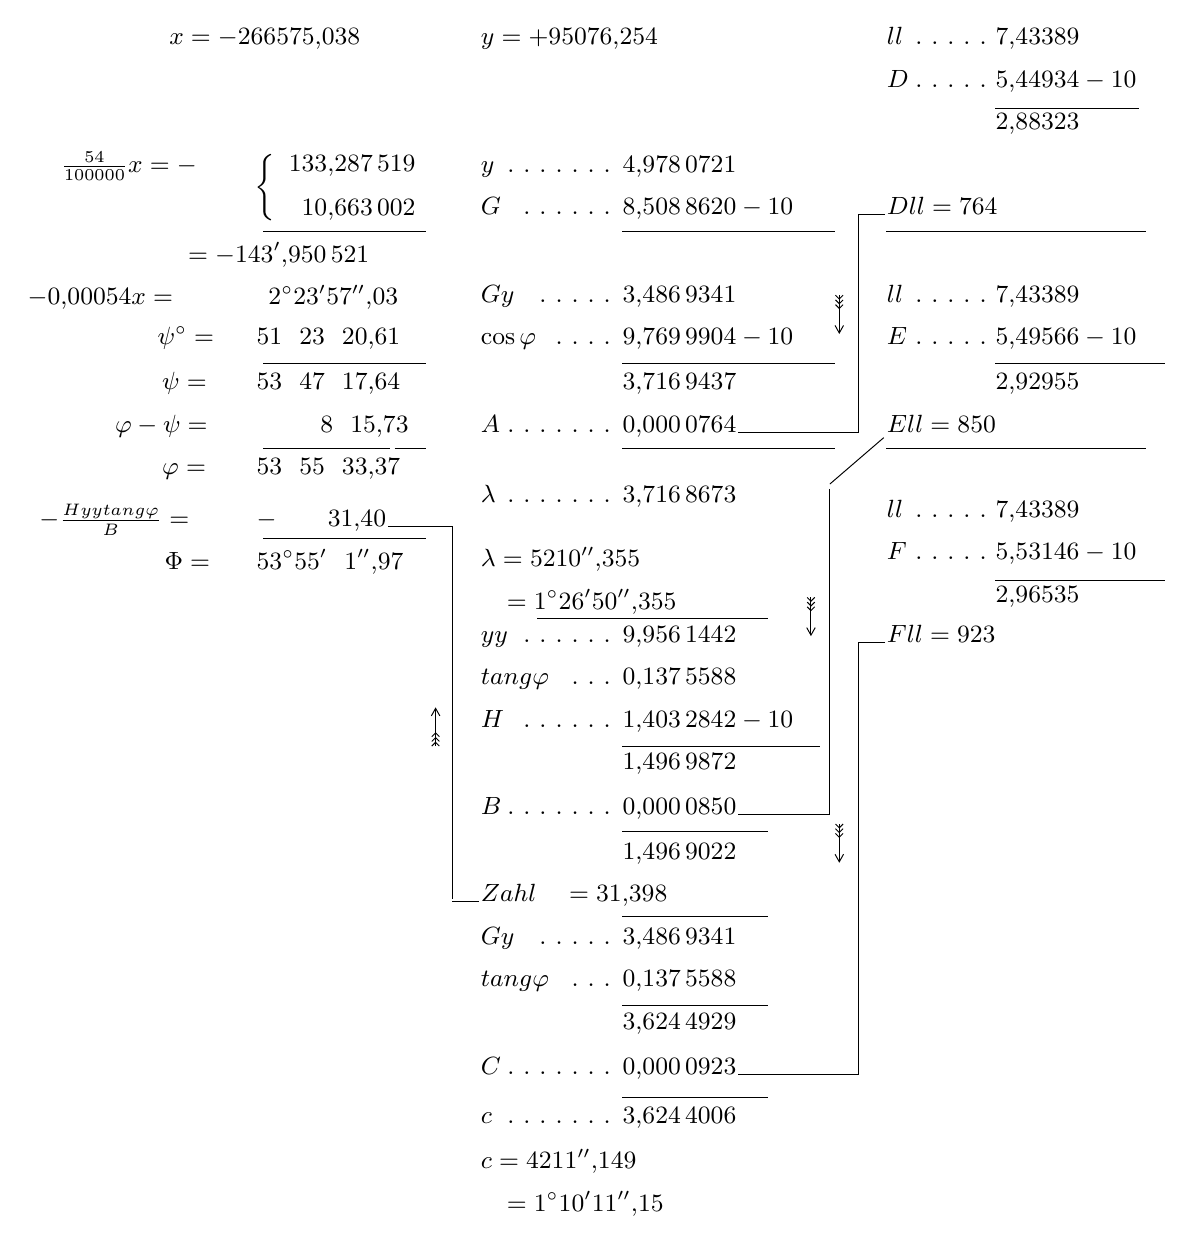
\begin{tikzpicture}[x=.006cm,y=-.006cm,every node/.style={anchor=base west,inner sep=0pt,font=\fontsize{8.8}{10}\selectfont},line width=.35pt]
\node at (280,60) {$x=-266575{,}038$};
\node at (940,60) {$y=+95076{,}254$};
\node at (50,330) {$\frac{54}{100000}x=-$};
\node at (460,375) {$\left\{\begin{array}{r}133{,}287\,519\\[5pt]10{,}663\,002\end{array}\right.$};
\draw (480,455) -- (825,455);
\node at (320,520) {$=-143'{,}950\,521$};
\node at (-20,610) {$-0{,}00054x=$};
\node at (490,610) {$2^\circ23'57''{,}03$};
\node at (255,695) {$\psi^\circ=$};
\node at (465,695) {$51\ \ 23\ \ 20{,}61$};
\draw (480,735) -- (825,735);
\node at (265,790) {$\psi=$};
\node at (465,790) {$53\ \ 47\ \ 17{,}64$};
\node at (165,880) {$\varphi-\psi=$};
\node at (600,880) {$8\ \ 15{,}73$};
\draw (480,915) -- (748,915);
\draw (758,915) -- (825,915);
\node at (265,970) {$\varphi=$};
\node at (465,970) {$53\ \ 55\ \ 33{,}37$};
\node at (5,1080) {$-\frac{Hyy\operatorname{tang}\varphi}{B}=$};
\node (PhiCorrection) at (465,1080) {$-\qquad31{,}40$};
\draw (480,1105) -- (825,1105);
\node at (270,1170) {$\Phi=$};
\node at (465,1170) {$53^\circ55'\ \ 1''{,}97$};
\node at (940,330) {$y$};
\node at (996,330) {$.$};
\node at (1030,330) {$.$};
\node at (1064,330) {$.$};
\node at (1098,330) {$.$};
\node at (1132,330) {$.$};
\node at (1166,330) {$.$};
\node at (1200,330) {$.$};
\node at (1240,330) {$4{,}978\,0721$};
\node at (940,420) {$G$};
\node at (1030,420) {$.$};
\node at (1064,420) {$.$};
\node at (1098,420) {$.$};
\node at (1132,420) {$.$};
\node at (1166,420) {$.$};
\node at (1200,420) {$.$};
\node at (1240,420) {$8{,}508\,8620-10$};
\node at (940,605) {$Gy$};
\node at (1064,605) {$.$};
\node at (1098,605) {$.$};
\node at (1132,605) {$.$};
\node at (1166,605) {$.$};
\node at (1200,605) {$.$};
\node at (1240,605) {$3{,}486\,9341$};
\node at (940,695) {$\cos\varphi$};
\node at (1098,695) {$.$};
\node at (1132,695) {$.$};
\node at (1166,695) {$.$};
\node at (1200,695) {$.$};
\node at (1240,695) {$9{,}769\,9904-10$};
\node at (940,880) {$A$};
\node at (996,880) {$.$};
\node at (1030,880) {$.$};
\node at (1064,880) {$.$};
\node at (1098,880) {$.$};
\node at (1132,880) {$.$};
\node at (1166,880) {$.$};
\node at (1200,880) {$.$};
\node (Aval) at (1240,880) {$0{,}000\,0764$};
\node at (940,1030) {$\lambda$};
\node at (996,1030) {$.$};
\node at (1030,1030) {$.$};
\node at (1064,1030) {$.$};
\node at (1098,1030) {$.$};
\node at (1132,1030) {$.$};
\node at (1166,1030) {$.$};
\node at (1200,1030) {$.$};
\node at (1240,1030) {$3{,}716\,8673$};
\node at (940,1325) {$yy$};
\node at (1030,1325) {$.$};
\node at (1064,1325) {$.$};
\node at (1098,1325) {$.$};
\node at (1132,1325) {$.$};
\node at (1166,1325) {$.$};
\node at (1200,1325) {$.$};
\node at (1240,1325) {$9{,}956\,1442$};
\node at (940,1415) {$\operatorname{tang}\varphi$};
\node at (1132,1415) {$.$};
\node at (1166,1415) {$.$};
\node at (1200,1415) {$.$};
\node at (1240,1415) {$0{,}137\,5588$};
\node at (940,1505) {$H$};
\node at (1030,1505) {$.$};
\node at (1064,1505) {$.$};
\node at (1098,1505) {$.$};
\node at (1132,1505) {$.$};
\node at (1166,1505) {$.$};
\node at (1200,1505) {$.$};
\node at (1240,1505) {$1{,}403\,2842-10$};
\node at (940,1690) {$B$};
\node at (996,1690) {$.$};
\node at (1030,1690) {$.$};
\node at (1064,1690) {$.$};
\node at (1098,1690) {$.$};
\node at (1132,1690) {$.$};
\node at (1166,1690) {$.$};
\node at (1200,1690) {$.$};
\node (Bval) at (1240,1690) {$0{,}000\,0850$};
\node at (940,1965) {$Gy$};
\node at (1064,1965) {$.$};
\node at (1098,1965) {$.$};
\node at (1132,1965) {$.$};
\node at (1166,1965) {$.$};
\node at (1200,1965) {$.$};
\node at (1240,1965) {$3{,}486\,9341$};
\node at (940,2055) {$\operatorname{tang}\varphi$};
\node at (1132,2055) {$.$};
\node at (1166,2055) {$.$};
\node at (1200,2055) {$.$};
\node at (1240,2055) {$0{,}137\,5588$};
\node at (940,2240) {$C$};
\node at (996,2240) {$.$};
\node at (1030,2240) {$.$};
\node at (1064,2240) {$.$};
\node at (1098,2240) {$.$};
\node at (1132,2240) {$.$};
\node at (1166,2240) {$.$};
\node at (1200,2240) {$.$};
\node (Cval) at (1240,2240) {$0{,}000\,0923$};
\node at (940,2345) {$c$};
\node at (996,2345) {$.$};
\node at (1030,2345) {$.$};
\node at (1064,2345) {$.$};
\node at (1098,2345) {$.$};
\node at (1132,2345) {$.$};
\node at (1166,2345) {$.$};
\node at (1200,2345) {$.$};
\node at (1240,2345) {$3{,}624\,4006$};
\node at (1240,790) {$3{,}716\,9437$};
\node at (1240,1595) {$1{,}496\,9872$};
\node at (1240,1785) {$1{,}496\,9022$};
\node at (1240,2145) {$3{,}624\,4929$};
\draw (1240,455) -- (1690,455);
\draw (1240,735) -- (1690,735);
\draw (1240,915) -- (1690,915);
\draw (1060,1275) -- (1550,1275);
\draw (1240,1545) -- (1660,1545);
\draw (1240,1725) -- (1550,1725);
\draw (1240,1905) -- (1550,1905);
\draw (1240,2095) -- (1550,2095);
\draw (1240,2290) -- (1550,2290);
\node at (940,1165) {$\lambda=5210''{,}355$};
\node at (995,1255) {$=1^\circ26'50''{,}355$};
\node (Zahl) at (940,1875) {$\text{Zahl}\quad=31{,}398$};
\node at (940,2440) {$c=4211''{,}149$};
\node at (995,2530) {$=1^\circ10'11''{,}15$};
\node at (1800,60) {$ll$};
\node at (1860,60) {$.$};
\node at (1894,60) {$.$};
\node at (1928,60) {$.$};
\node at (1962,60) {$.$};
\node at (1996,60) {$.$};
\node at (2030,60) {$7{,}43389$};
\node at (1800,150) {$D$};
\node at (1860,150) {$.$};
\node at (1894,150) {$.$};
\node at (1928,150) {$.$};
\node at (1962,150) {$.$};
\node at (1996,150) {$.$};
\node at (2030,150) {$5{,}44934-10$};
\node at (1800,605) {$ll$};
\node at (1860,605) {$.$};
\node at (1894,605) {$.$};
\node at (1928,605) {$.$};
\node at (1962,605) {$.$};
\node at (1996,605) {$.$};
\node at (2030,605) {$7{,}43389$};
\node at (1800,695) {$E$};
\node at (1860,695) {$.$};
\node at (1894,695) {$.$};
\node at (1928,695) {$.$};
\node at (1962,695) {$.$};
\node at (1996,695) {$.$};
\node at (2030,695) {$5{,}49566-10$};
\node at (1800,1060) {$ll$};
\node at (1860,1060) {$.$};
\node at (1894,1060) {$.$};
\node at (1928,1060) {$.$};
\node at (1962,1060) {$.$};
\node at (1996,1060) {$.$};
\node at (2030,1060) {$7{,}43389$};
\node at (1800,1150) {$F$};
\node at (1860,1150) {$.$};
\node at (1894,1150) {$.$};
\node at (1928,1150) {$.$};
\node at (1962,1150) {$.$};
\node at (1996,1150) {$.$};
\node at (2030,1150) {$5{,}53146-10$};
\node at (2030,240) {$2{,}88323$};
\node at (2030,790) {$2{,}92955$};
\node at (2030,1240) {$2{,}96535$};
\node (Dll) at (1800,420) {$Dll=764$};
\node (Ell) at (1800,880) {$Ell=850$};
\node (Fll) at (1800,1325) {$Fll=923$};
\draw (2030,195) -- (2335,195);
\draw (1800,455) -- (2350,455);
\draw (2030,735) -- (2390,735);
\draw (1800,915) -- (2350,915);
\draw (2030,1195) -- (2390,1195);
\draw ([xshift=-.5pt]Dll.base west) -- (1740,420) -- (1740,880) -- ([xshift=.5pt]Aval.base east);
\draw ([xshift=-1pt,yshift=-2pt]Ell.base west) -- (1680,990);
\draw (1680,1000) -- (1680,1690) -- ([xshift=.5pt]Bval.base east);
\draw ([xshift=-.5pt]Fll.base west) -- (1740,1325) -- (1740,2240) -- ([xshift=.5pt]Cval.base east);
\draw ([xshift=.5pt]PhiCorrection.base east) -- (880,1080) -- (880,1868);
\draw (880,1875) -- ([xshift=-.5pt]Zahl.base west);
\draw (1700,590) -- (1700,670);
\draw (1691,654) -- (1700,670) -- (1709,654);
\draw (1692,590) -- (1700,598) -- (1708,590);
\draw (1692,600) -- (1700,608) -- (1708,600);
\draw (1692,610) -- (1700,618) -- (1708,610);
\draw (1640,1230) -- (1640,1310);
\draw (1631,1294) -- (1640,1310) -- (1649,1294);
\draw (1632,1230) -- (1640,1238) -- (1648,1230);
\draw (1632,1240) -- (1640,1248) -- (1648,1240);
\draw (1632,1250) -- (1640,1258) -- (1648,1250);
\draw (1700,1710) -- (1700,1790);
\draw (1691,1774) -- (1700,1790) -- (1709,1774);
\draw (1692,1710) -- (1700,1718) -- (1708,1710);
\draw (1692,1720) -- (1700,1728) -- (1708,1720);
\draw (1692,1730) -- (1700,1738) -- (1708,1730);
\draw (845,1545) -- (845,1465);
\draw (836,1481) -- (845,1465) -- (854,1481);
\draw (837,1545) -- (845,1537) -- (853,1545);
\draw (837,1535) -- (845,1527) -- (853,1535);
\draw (837,1525) -- (845,1517) -- (853,1525);
\end{tikzpicture}
\end{center}
\vfill\hfill$27^*$\hspace*{2cm}\par
\endgroup
